%%%%%%%%%%%%%%%%%%%%%%%%%%%%%%%%%%%%%%%%%%%%%%%%%%%%%%%%%%%%%%%%%%%%%%%%%%%%%%%%%%%%%%%%%
% Section 9: Example Programs
%	This section describes several example programs in the RapidSmith2 repository that
%	can be used to learn how to use RapidSmith2.
%%%%%%%%%%%%%%%%%%%%%%%%%%%%%%%%%%%%%%%%%%%%%%%%%%%%%%%%%%%%%%%%%%%%%%%%%%%%%%%%%%%%%%%%%
\newpage
\section{Example Programs} \label{examples}
\graphicspath{{./techReportFigures/sec9_examples/}}

A variety of example programs can be found in the
\pkg{edu.byu.edu.rapidSmith.examples} package of the RapidSmith2 installation.
They have been heavily commented to provide a means to learn the RapidSmith2 API by
example. We believe this approach is better than reading through a block of
text while trying to understand the data structures and what they do.
There is a \fil{README.txt} file in that directory to provide an overview of
each example. The order that they appear in the \fil{README.txt} is also the
suggested learning order for beginners. In addition, the subsections below
describe one or more built-in RapidSmith2 programs which you might find useful.

\subsection{Sample Vivado Designs}
To enable new users of RapidSmith2 to quickly start running the example
programs, a small set of pre-compiled Vivado designs have been included in the
distribution. They are located in the \dir{exampleVivadoDesigns} directory of
the repository, and consist of 3 designs: 
\begin{itemize}
\item \textbf{add.rscp}: synthesized only
\item \textbf{cordic.rscp}: synthesized and placed
\item \textbf{count16.rscp}: synthesized, placed and routed
\end{itemize} 
Equivalent Vivado checkpoints files (.dcp) are also included in
the same directory as \fil{add.dcp}, \fil{cordic.dcp}, and \fil{count16.dcp}
files. To open these checkpoints in Vivado, you can either (a) double click on
the .dcp file in a file explorer, or (b) use the command
\texttt{open\_checkpoint} when a Vivado terminal is open. It is suggested that
you have the equivalent Vivado designs open when going through the example
programs listed below.

If you want to recompile the designs from scratch, the source code for each
design has also been included in the same directory. The Tcl script called
\pgm{compile.tcl} can be used for this purpose. Simply open Vivado in Tcl
mode, and type the Tcl commands shown in \autoref{lst:compilation} to re-compile
and implement one of the example designs. This will synthesize, place, and
route a design and, from that compiled design, generate the \dir{.rscp}
directory and the \fil{.dcp} file. For example programs that only explore the
architecture, opening the device browser in Vivado can also be helpful.
                 
\begin{lstlisting} [numbers=none,keywordstyle=\ttfamily, caption=Sample
Tcl commands to run the Vivado compilation script, label=lst:compilation] 
	Vivado% cd <path to exampleVivadoDesigns directory>
	Vivado% source compile.tcl
	Vivado% compile_hdl_to_checkpoint_files add
	Vivado% close_project
\end{lstlisting}

\subsection{\pgm{DeviceBrowser}}
The DeviceBrowser is a GUI program located in the 
\pkg{edu.byu.ece.rapidSmith.device.browser} package. It lets you browse
parts at the tile level, and is useful for becoming more familiar with FPGA
architecture. As long as a valid device file exists, then the DeviceBrowser can
operate (no design required). A screenshot from the DeviceBrowser can be seen in
\autoref{fig:deviceBrowser}. On the left, the user may choose the desired part
by navigating the tree menu and double-clicking on the desired part name.
This will load the part in the viewer pane on the right (the first available
part is loaded at startup). The status bar in the bottom left displays which
part is currently loaded. Also displayed is the name of the current tile
which the mouse is over, highlighted by a yellow outline in the viewer pane.
The user may navigate inside the viewer pane by using the mouse. By
right-clicking and dragging the cursor, the user may pan. By using the
scroll-wheel on the mouse, the user may zoom. If a scroll-wheel is
unavailable, the user may zoom by clicking inside the viewer pane and pressing
the minus(-) key to zoom out or the equals(=) key to zoom in.

\begin{figure}[htb]
\centering
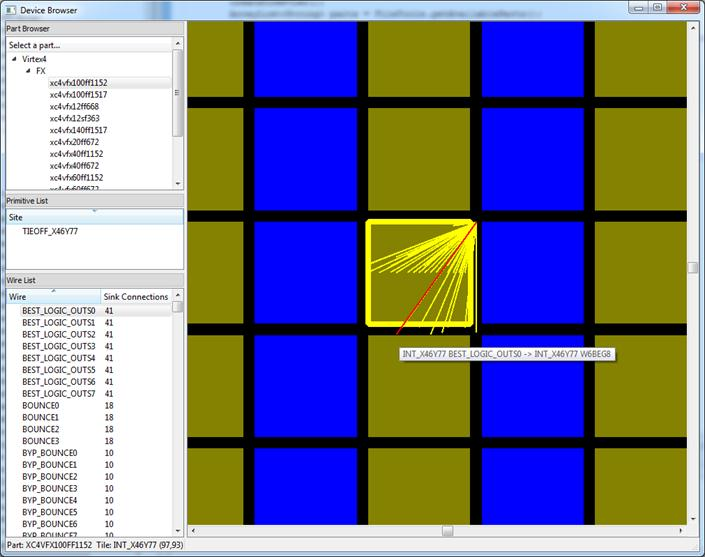
\includegraphics[width=0.8\columnwidth]{deviceBrowser2.jpg}
\caption{\pgm{DeviceBrowser} Screen Shot Showing Wire Connections}
\label{fig:deviceBrowser2}
\end{figure}

The device browser also allows the user to follow the various connections found
in the FPGA.  By double clicking a wire in the wire list, the application will
draw the connection on the tile array (as shown in
\autoref{fig:deviceBrowser2}). By hovering the mouse pointer over the
connection, the wire becomes red and a tooltip will appear describing the
connection made by declaring the source tile and wire followed by an arrow and
the destination tile and wire.  By clicking on the wire, the application will
redraw all the connections that can be made from the currently selected wire. 
By repeating this action, the user can follow connections and discover how the
FPGA interconnect is laid out. Thanks to Chris Lavin for originally creating
this application.

\subsection{\pgm{DeviceAnalyzer}}
The DeviceAnalyzer is designed as a simple getting started program and
demonstrates how to use some of the Device data structures in RapidSmith2. This
includes how to query for and print tiles in a device, how to use wires and
wire connections, and other useful device functions.

\subsection{\pgm{ImportExportExample}} \label{sec:importExportExample}
The ImportExportExample demonstrates how to load a RapidSmith Checkpoint
(RSCP) into RapidSmith2, and how to export a RapidSmith2 design back into a Tincr
Checkpoint (TCP). This is a very important step in passing digital designs back
and forth between Vivado and RapidSmith2.

\subsection{\pgm{DesignAnalyzer}}
The DesignAnalyzer loads a RapidSmith Checkpoint into RapidSmith2, walks
the design data structures, and prints what it finds as it goes in a
readable format. As such, it provides a nice example of a number of things which would
be useful for getting started with RapidSmith2 including:
\begin{itemize}
  \item How to enumerate the Cells in a design, determine and print their 
  placement information, and determine and print their properties.
  \item How to enumerate the logical nets in a design and print out their source
  and sink pins. 
  \item How to traverse and print out the physical route for a logical net (if
  it is routed)  
\end{itemize}

\subsection{CreateDesignExample} \label{sec:createDesignExample}
The CreateDesignExample program builds a RapidSmith2 netlist from scratch (using
\cells and \cellnets) and then places the design. While this is certainly not
recommended for substantial designs, it does demonstrate how to do the
following useful tasks in RapidSmith2:

\begin{itemize}
  \item Create new \cells and add them to an existing netlist
  \item Create new \cellnets, and connect them to \cls{CellPin}s
  \item Modify the properties on \cells
  \item Place \cells onto a \bels
  \item Find compatible \bel placement for a given \cell
\end{itemize}

\subsection{Other Test Programs}
The programs introduced in this section are designed for beginners of RapidSmith2. Once
you start becoming more comfortable with RapidSmith2 and its data structures,
there are several other more advanced examples. These examples include the
\pgm{HandRouter}, \pgm{AStarRouter}, and \pgm{SimulatedAnnealingPlacer}
programs. See the README.txt file for more information about each of these
examples.
